\chapter{Overall Description}

This chapter contains a general description of the system from a high level point of view. \\
It describes the general factors that affect the product and its requirements. It does not state specific requirements. Instead, it provides them a background, which is useful to define them in detail in \textit{Chapter 3}.\\
Starting from scenarios and domain models, it proceeds with an analysis of product functions and users' most relevant needs in order to define assumptions, dependencies and constraints of the entire application system.



\section{Product Perspective}
In subsection \textit{2.1.1} are listed the most relevant scenarios which are a narrative description of what users do and experience as they try to make use of the application.\\
They provide a general depiction of how major components of the system and users interact.\\
Moreover, in subsections \textit{2.1.2} and \textit{2.1.3} the domain of the system is defined through different models using UML.

\subsection{Scenarios}

\begin{enumerate}

\item Scenario: \textbf{Sunil discovers DREAM}\\\\
Sunil is a farmer from Telangana. Unfortunately, due to the adverse and unpredictable effects of climate change, his production of black carrots is gradually decreasing. Sunil learns from a colleague of his that there is an application called DREAM that could help him. Sunil registers and logs in, hoping to profit from it and improve his production.\\

\item Scenario: \textbf{Rajesh looking for advice}\\\\
Rajesh is a landowner from Adilabad district in Telangana, he owns several agricultural properties in the city. After his recent business trip to Russia, where he attended the beet fair, he is convinced to plant beets on his land too. As this is a little-known plant in the area, he doesn't know who to ask for advice. Rajesh's son Ram, also in the agricultural sector for several years, advises his father to use DREAM since Rajesh already had an account registered with the application.
Rajesh consults on the application the discussions already opened by other Telangana farmers to see if any of them had ever sought advice on beet cultivation. Unfortunately he cannot find any, so thanks to the suggestion of his son Ram he decides to open a thread on the dedicated forum, so that he can ask for advice about the plant from other farmers throughout Telangana.\\

\item Scenario: \textbf{Anita and her strategic plan}\\\\
Anita is the administrator of her mandal Sarangapur, in Jagtial district, as an inspector of production and development of the primary sector. Sarangapur is characterized by great periods of drought, so water is a particularly precious resource for citizens.
Recent analyzes have shown that over 90\% of the water is used by farmers.
Anita discovers DREAM and she wants to monitor the water consumption within each mandal in Telangana over the current year. Her goal is to identify the one that consumes the least water to study its strategies, so she enters the parameters of interest (quantity of water and Telangana mandals) on the application.
At this point the app returns the mandals and the corresponding consumed water in this last year and Anita is pleased to discover that the primacy is Pegadapalli, a mandal from her own district.\\

\item Scenario: \textbf{Manoj, the Indian tycoon}\\\\
Manoj is an Indian tycoon who would like to invest his capital in the agricultural sector. He accesses the DREAM application as policy maker and checks the map showing the performance score of each mandal. Manoj identifies the best performing ones and decides to invest in Geesugonda mandal which is located in Warangal district.\\

\item Scenario: \textbf{Mahima is thrilled with joy for DREAM}\\\\
Mahima is the Additional Director of Agriculture who assist the state Head quarter Commissioner\&Director of Agriculture in Telangana. She belongs to the Department of Agriculture, which provides agricultural services to farmers and aims to transfer the latest technical knowledge to the farming community. She was one of those who pushed for the creation of DREAM.
Mahima is thrilled with joy for its market launch and she is looking forward to use the application, therefore she gets her personal ID code to be able to registers with the role of policy maker and logs into DREAM.\\

\item Scenario: \textbf{A new job for Shanti}\\\\
Shanti is a young agronomist who operated in Palakeedu, a mandal in Suryapet district. She sees the announcement published on the Telangana government website in which it is reported that the DREAM application has been launched on the market and that for each mandal is required an agronomist. She is unemployed and interested in filling this role. Therefore, she sends her CV, gets hired and receives her personal ID code which allows her to register into DREAM. Eventually, she inserts Palakeedu as mandal of her competence.\\

\item Scenario: \textbf{Champak tries natural farming}\\\\
Champak is a farmer who has planted wheat. The last crop was poor because he didn't have enough money to buy suitable pesticides. He still can't afford them, however he cannot suspend his agricultural activity since his family depends on it as the principal means of livelihood. For this reason Champak creates a help request to both the agronomist and well performing farmers. The first to answer is Jayapal, a well performing farmer from his same mandal. Jayapal suggests him to plant potatoes instead of wheat because they are more resistant. However, Champak has already planted wheat therefore changing crops is out of the question. Champak waits for other answers until Rajat, the agronomist, replies suggesting him to cover the seeds with microorganisms obtained from particular formulations of cow dung. Champak is willing to follow the advice and is satisfied with the answer. He marks the help request as solved. 
\\

\item Scenario: \textbf{The busy life of Aruna}\\\\
Aruna is the DREAM agronomist responsible for Jaipur mandal in Mancherial district. It is early morning and the working day is about to begin. Aruna consults the daily plan to check which are the scheduled visits for the day. An appointment with the farmer Gangesh is scheduled for the afternoon. At that moment she receives a phone call from him, who informs her that his wife is not well, he has to take her to the doctor and for this he has to cancel the scheduled visit. Aruna wishes him the best and updates the daily plan, cancelling the appointment. Further on, she completes all the appointments scheduled in the morning and she drives her car to reach Jaya, a farmer. Unfortounately, Aruna has a small accident with her car, she is unharmed but she will miss the appointment. She informs Jaya and calls a mechanic. She finally returns home in the evening and confirms the daily plan, also specifying the deviation corresponding to the missed visit due to the accident. She also has to reschedule in the first two free slots in her agenda the appointments with Jaya and Gangesh. To do so, she updates the daily plan of the next day. 
\\
\item Scenario: \textbf{Durvish, the inspector}\\\\
Durvish is the administrative head of Doma mandal, in Vikarabad district. The DREAM application was launched on the market the year before and now he wants to understand whether the steering initiatives carried out by agronomists with the help of good farmers have produced significant results. Therefore, Durvish accesses DREAM with his account and he enters the parameters of interest on the application to select only farmers of his mandal with at least an Help Request solved.
At this point the app returns the selected farmers. Durvish wants to visualize their general trend of the performance score as indicator of the efficiency of the application. He selects score as attribute and mean as operation, in return a time chart is shown. He pleasantly discovers that, except for an initial fluctuating trend, the general performance score of farmers with at least a solved Help Request of his mandal is constantly growing, a sign of effective usefulness of DREAM.
\\

\item Scenario: \textbf{Deepa fights soil salinity}\\\\
Deepa is a farmer of Telangana who is already using the application DREAM. The cotton she planted is now ready for harvest. The amount of cotton obtained from her hectare of land results in 3 bales, which correspond approximately to 107 kg each. Deepa accesses the app, selects the date corresponding to the current day and inserts in the system type and quantity of product harvested. Two days later, while approaching to plant cotton seeds again, she has a problem regarding the salinity of the soil which is particularly high and would not allow cotton to grow. For this reason, Deepa stores this information in the system selecting the current day, also adding that it was necessary to buy a biostimulant whose formulation neutralizes excess salts within the soil.
\\

\item Scenario: \textbf{Haresh's first encounter with coffee}\\\\
Haresh is a farmer of Telangana who is already using the application DREAM. It is October and within a few days he will have to harvest the sorghum he has planted. To better organize the work of the next few days, Haresh accesses the application and checks the weather forecasts. After the harvest he will also have to decide what to plant, which is why he also checks the soil moisture. Furthermore, due to the drought expected for November, the app suggests Haresh to plant coffee, a product that does not require a particularly humid soil. Haresh thinks that it could be a good idea, however he has never cultivated coffee so it could be necessary to confront with the agronomist about some technical details. Haresh doesn't remember when his next visit with the agronomist will occur, therefore he accesses the visits page on the application and pleasantly reads that one is scheduled for November 5th.
\\

\item Scenario: \textbf{Lohit helps the most needy}\\\\
Lohit is the DREAM agronomist responsible for Raipole mandal in Siddipet district. The performance score in his mandal for a good percentage of farmers has been around a value that has not been particularly high for more than six months. For this reason Lohit wants to visualize data regarding best performing farmers to formulate strategies to be applied to the most needy. He accesses DREAM and visualizes farmers whose performance score is between the highest. Analyzing the corresponding data he finds out that they cultivate all the same type of product: rice, which is cultivable under widely varying conditions but prefers hot and humid climate. Therefore, before advising other farmers to plant rice, Lohit consults weather forecasts and humidity of soil trend, discovering that with a very high probability there will be the perfect conditions in the next weeks.
\\

\end{enumerate}

\newpage
\subsection{Class Diagram}
In this section is reported the Class Diagram of the System, whose main concepts are presented from a high-level point of view. 
\begin{figure}[H]
  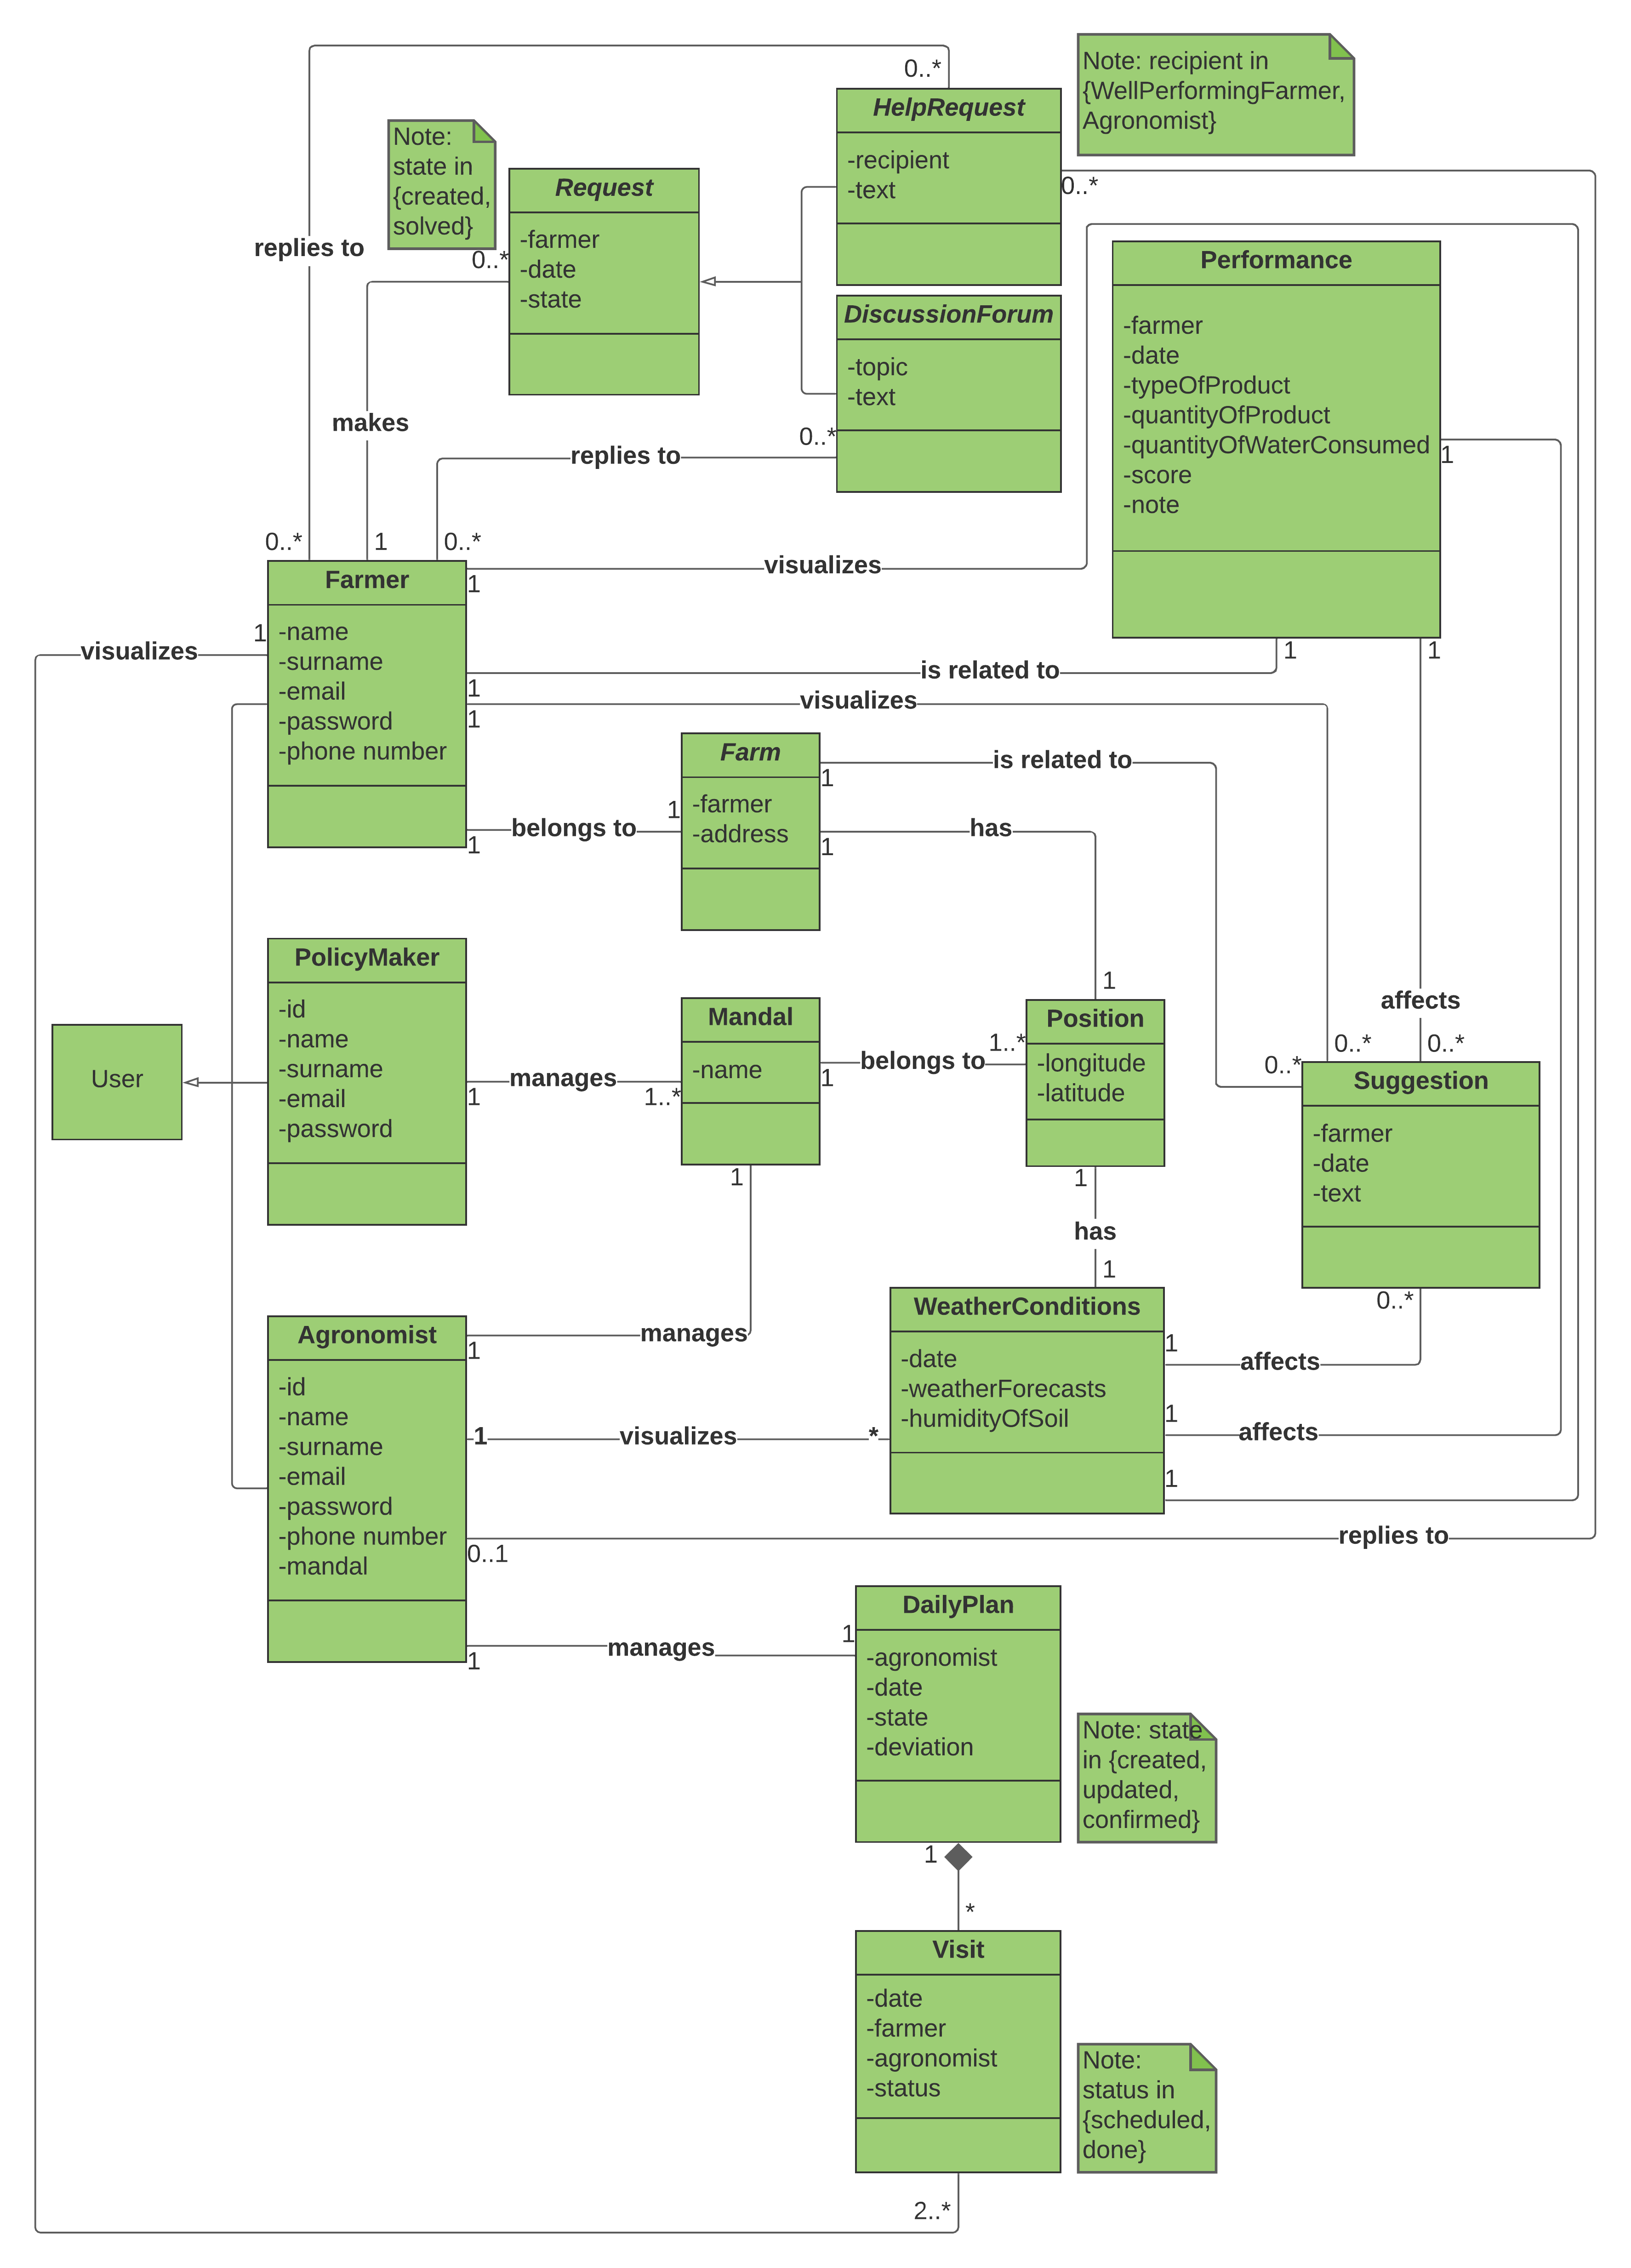
\includegraphics[width=125.5mm,scale=0.9]{./Images/Class Diagram DREAM.png}
  \caption{Class Diagram}
\end{figure}





\newpage



\subsection{State Charts}

\subsubsection{Daily Plan State Diagram}
This state diagram shows the three states of a Daily Plan.\\
The Daily Plan is \textit{Created} by the system and then \textit{Updated} or carried out and \textit{Confirmed} by the agronomist, depending on whether he needs to change the plan or not.
\begin{figure}[h!]
  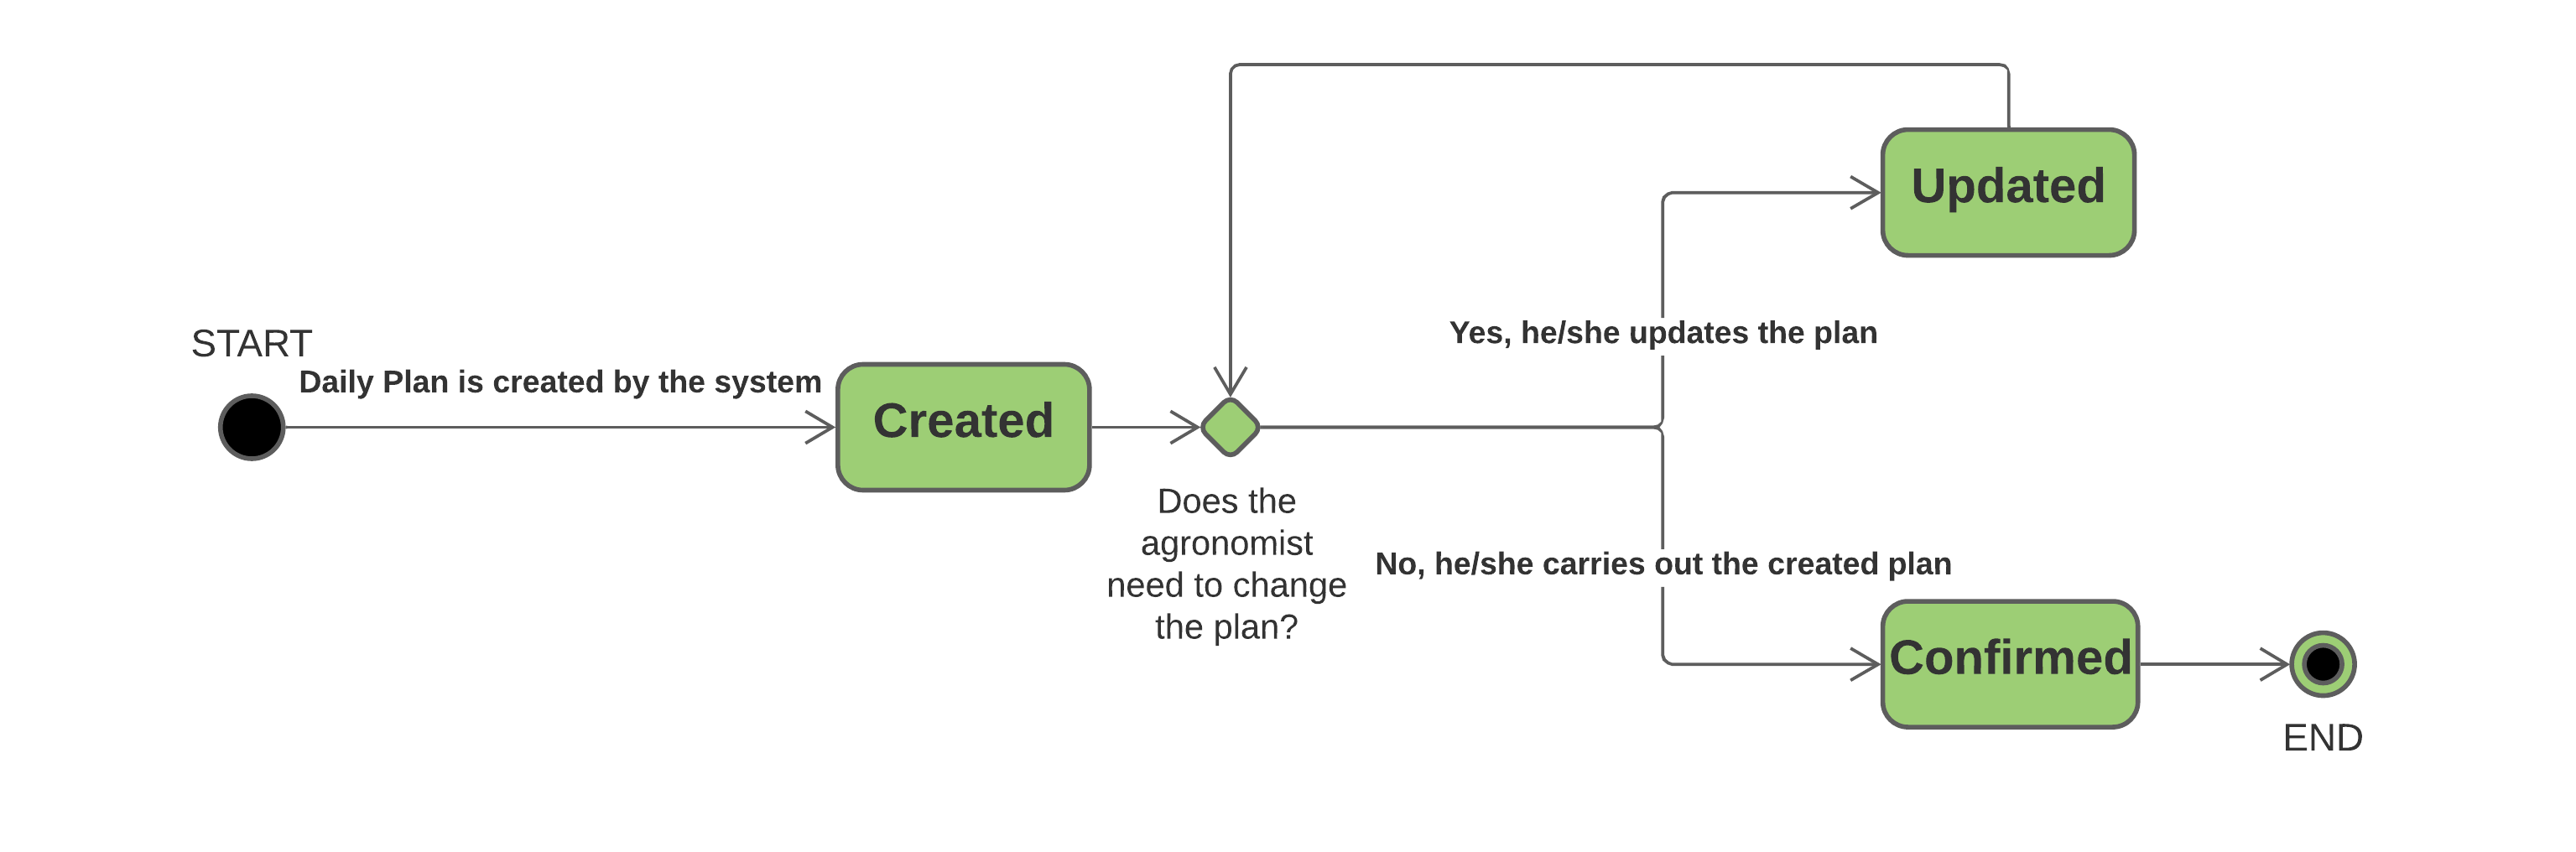
\includegraphics[width=\textwidth,height=\textheight,keepaspectratio]{./Images/State Chart DailyPlan.png}
  \caption{Daily Plan State Diagram}
\end{figure}

\subsubsection{Help Request State Diagram}
This state diagram shows the two states of a Help Request.\\
The Help Request is \textit{Created} and then \textit{Solved} by the farmer, depending on whether he is satisfied with the reply received or not.
\begin{figure}[h!]
  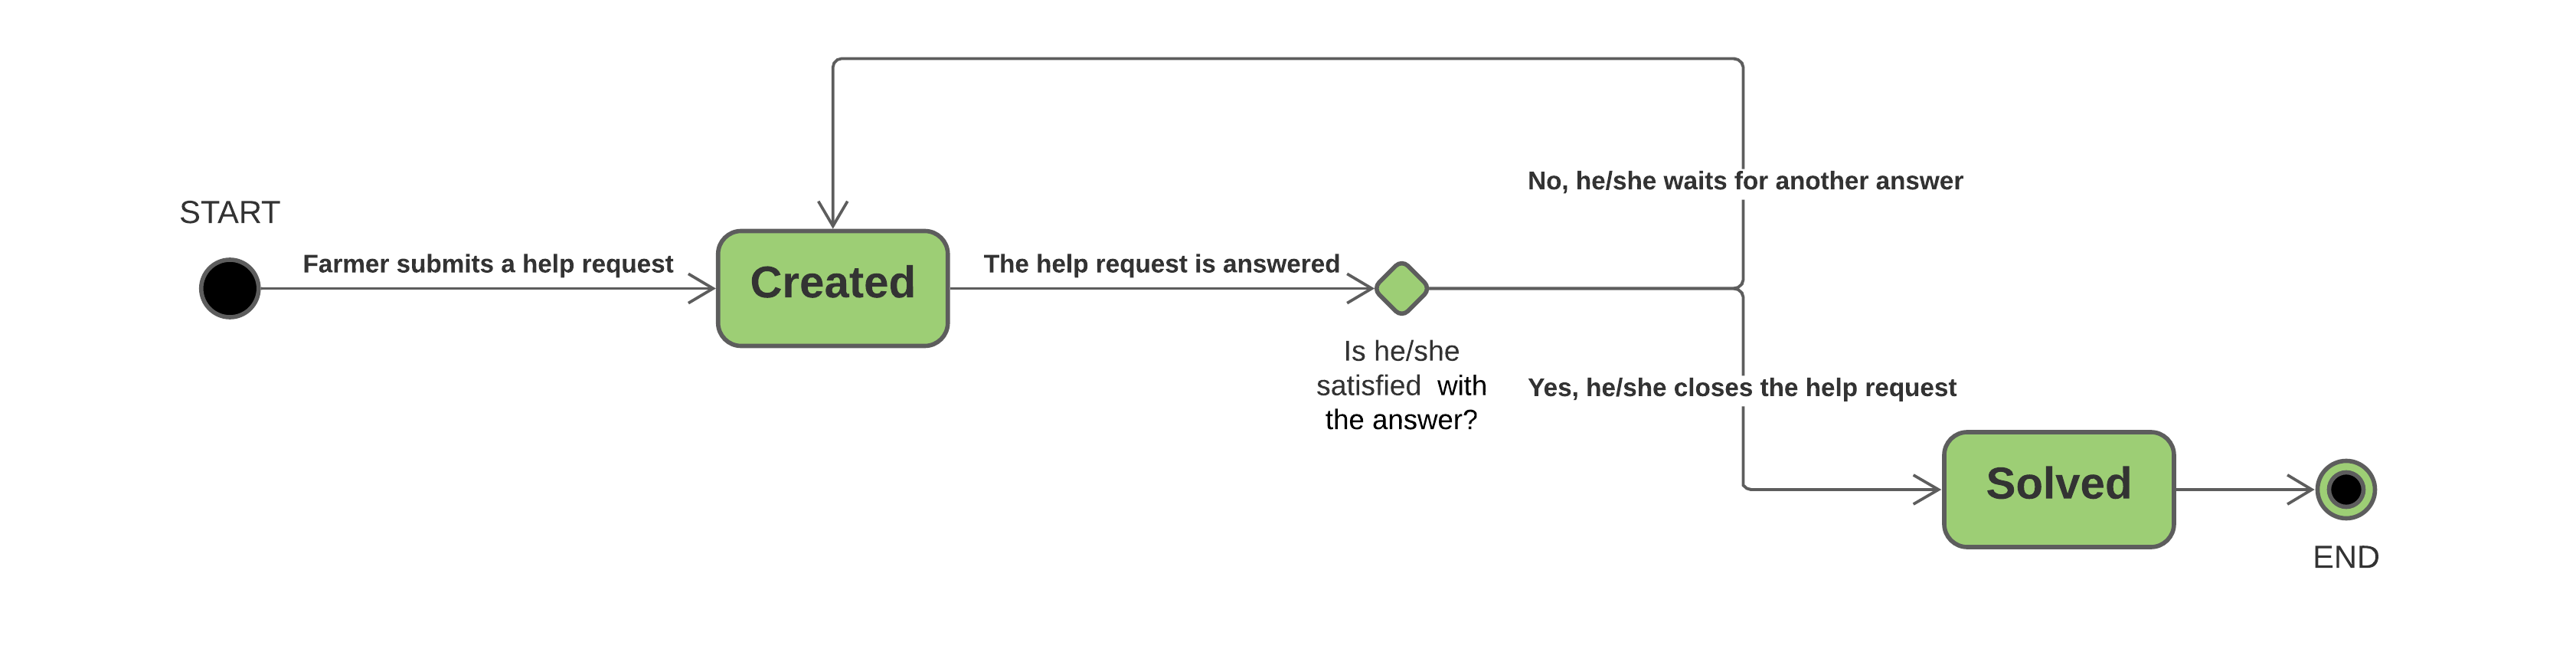
\includegraphics[width=\textwidth,height=\textheight,keepaspectratio]{./Images/State Chart HelpRequest.png}
  \caption{Help Request State Diagram}
\end{figure}

\subsubsection{Discussion Forum State Diagram}
This state diagram shows the two states of a Discussion Forum.\\
The Discussion Forum is \textit{Created} and then \textit{Solved} by the farmer, depending on whether he is satisfied with the replies received or not.
\begin{figure}[h!]
  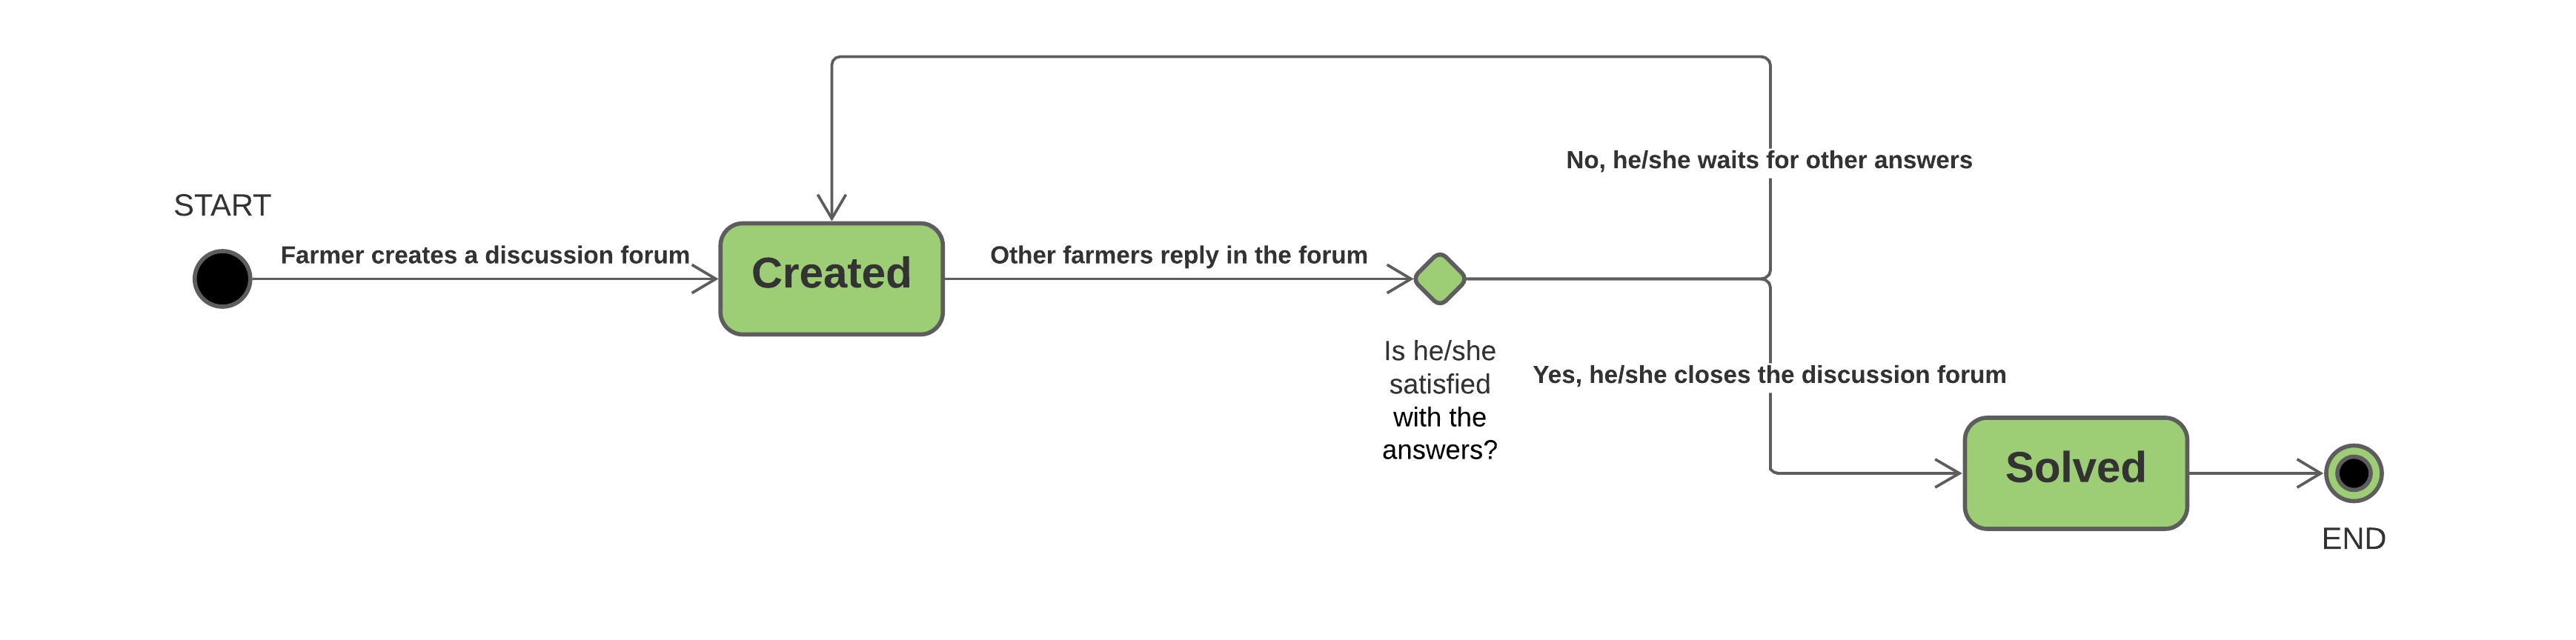
\includegraphics[width=\textwidth,height=\textheight,keepaspectratio]{./Images/State Chart DiscussionForum.png}
  \caption{Discussion Forum State Diagram}
\end{figure}

\subsubsection{Visit State Diagram}
This state diagram shows the two states of a Visit.\\
The Visit is \textit{Scheduled} and then \textit{Done} after the agronomist carries out the visit and confirms the corresponding Daily Plan.
\begin{figure}[h!]
  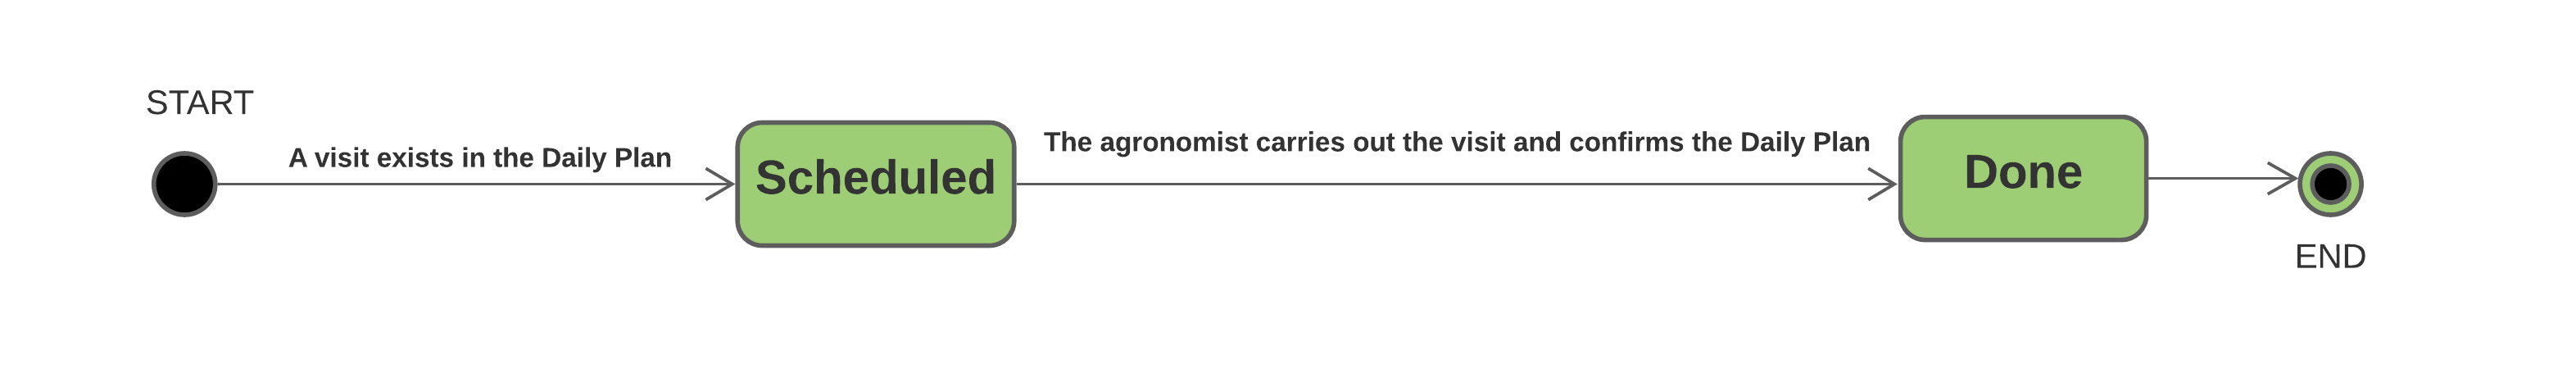
\includegraphics[width=\textwidth,height=\textheight,keepaspectratio]{./Images/State Chart Visit.png}
  \caption{Visit State Diagram}
\end{figure}

\section{Product functions}

\subsection{Registration}
In order to use the application all the actors (policy makers, agronomists and farmers) must be registered. The registration of an account can be performed in two ways: through the Web Application on a computer or through the mobile application on a smartphone.

In the case of the Web application, the farmer opens the web application and clicks on the "Register" button on the homepage. At this point he is redirected to the registration page where the farmer is asked to select which category of users he belongs to: "Policy Maker", "Farmer" or "Agronomist".
After selecting the right category he can enter in the predetermined fields the required data which in the case of the farmer are: name, surname, email, password, telephone number and his farm's address. The format of the characters entered is checked so that it complies with the predetermined rules of good formatting. 
If the rules on well-formed text are respected, a "Register now!" button appears. By clicking on it, the farmer is redirected to a new page that suggests to check his mailbox, where he will find an email generated and sent automatically by the system and with which the farmer can confirm his email by clicking on a link. After that the farmer is redirected to the login page in the Web app. The farmer then receives an email confirming his registration to DREAM.\\

Registration through the mobile application takes place in the same way as above. In fact, the farmer opens the application previously downloaded on his device. On the home page he clicks on the "Register" button. At this point he is redirected to the registration page where he can enter his data. The registration process continues as previously explained.\\

Registration takes place in the same way for all three actors, but there are some differences in the required data depending on the account role of the person who is registering. The data that agronomists and policy makers can enter are the same as those required by a farmer, with the exception of the farm's address.
The latter two roles (agronomists and policy makers) must enter an ID code assigned to them by the Telangana government to gain access to the system with their specific role after it is validated.
Moreover, only agronomists also have to inserts the mandal they are responsible of.


\subsection{Help Request}
DREAM allows farmers to make help request to the agronomist or even to well performing farmers if specified. The farmer accesses to the page "Help Request" and clicks on "Create a Help Request" button and accesses the corresponding page in which, in addition to the agronomist provided by default, he can select as recipient even well performing farmers of his/her same mandal. Eventually the farmer completes the text form corresponding to the body of the help request. Once finished, he/she confirms clicking on the correlated button "Confirm" and the help request is created. The help requests created by each farmer can be visualized by themselves accessing the page "Help Request" and clicking in the button "My Help Request". If someone replies the farmer visualizes in the same page the answer with the associated question \textit{"Are you satisfied with the answer?"} and the corresponding two possible answers \textit{"Yes"} or \textit{"No"}. Whether he/she is satisfied or not, he/she can:
\begin{enumerate}
    \item close the help request clicking on the button "Yes"
    \item not close it clicking on the button "No", waiting to receive other answers
\end{enumerate}
On the other hand, the users who can reply to a help request are the agronomist and well performing farmers of the same mandal. When a help request is created and they are mentioned among its recipients, they can visualize it in the "Help Request" page , where it is listed among the existing others. For each one there is a button "Answer" which they can click on to reply to the request.\\
Once the help request is solved by the farmer who made it, recipients cannot visualize it anymore. 

\subsection{Discussion Forum}
DREAM allows farmers to open a thread on the discussion forum. The farmer accesses the page "Discussion forum" and clicks on the button "Open a thread". He is redirected to a form which he fills in with topic and text and then he confirms. \\
The farmer can also look for a certain topic: he accesses the page "Discussion forum" and clicks on the button "Find a topic", the system provides him a form to fill in with the topic to be found and eventually it provides the farmer the list of existing associated threads.\\
If he wants to reply to one of them he can click on it and then, after pressing the button "Answer", he is redirected to a form in which he has to fill in the text's field. Eventually he confirms.

\subsection{Daily Plan}
DREAM allows agronomists to update the daily plan. He accesses the page "Daily Plan" and clicks on the button "Update". He is redirected to a form which he fills in with date (day and hour) and farmer and then he confirms. \\
The agronomist can also confirm the daily plan at the end of the day: he accesses the page "Daily Plan" and clicks on the button "confirm". He is redirected to a form with a field called "deviations" to be filled in only if modifications have been applied to the daily plan carried out during the day. Eventually he confirms.

\subsection{Notifications}
The system provides the farmer notifications regarding to: 
\begin{itemize}
    \item suggestions according to  his/her relevant information regarding his/her production and his/her farm's position
    \item new visits scheduled in the daily plan regarding him/her
    \item replies to his/her own help requests not yet solved
    \item replies to his/her own threads opened on the Discussion Forum
\end{itemize}
The agronomist and only well performing farmers are also provided with notifications regarding to new help requests received.\\

The actors involved can view the notification area directly from their homepage by clicking on the notification icon. At this point the actor is able to view all the notifications received in chronological order.

\subsection{Farmer inserts data regarding his production}
The farmer is allowed to enter relevant data about his production. Through his home page he has the possibility to insert new data on his harvest.
The data that the farmer has to enter in the form are: type of product and quantity of product collected. In addition, the farmer is allowed to add notes as well.\\
The system will add the current date of the insertion, the identification of the farmer (the email that uniquely identifies him) and the quantity of water consumed, information obtained thanks to some sensors.
After entering these data, the system will update the score for the farmer taking into account the new parameters entered.
The data entered will be saved in the database.


\section{Users Characteristics}
The actors of the applications are the following:
\begin{itemize}
    \item \textit {Policy maker}: he is an institutional figure in the public or private sector who has the power to elaborate and determine guidelines and strategies on the most relevant issues for society and politics. \textcolor{red}{He is registered into the application.}
    \item \textit {Agronomist}: he is a multidisciplinary professional figure. He works in favor of farms and small farmers by analyzing and developing projects based on direct observation and on the study of the best environmental solutions in order to improve productivity and enhance agricultural products. \textcolor{red}{He is registered into the application.}
    \item \textit {Farmer}: he is the figure who deals with managing, carrying out and producing crops of different kinds and types, constantly taking care of their good health. Furthermore, the farmer ensures that the places where the cultivation takes place fully comply with the hygienic-sanitary rules of the cultivation. They also provide for the maintenance of the structures necessary for the activities and the reclamation of the environments in which the cultivation takes place. \textcolor{red}{He is registered into the application.}
    \item \textit {Unregistered user}: a person who has not yet registered and is only allowed to sign up becoming either a Policy maker or an Agronomist or a Farmer depending on the type of membership.
\end{itemize}
\section{Assumptions, dependencies and constraints}

This subsection of the RASD lists each of the factors that affect the requirements stated in \textit{Chapter 3}.\\

An assumption is something that is believed to be true and which is outside of the project team’s control. Unlike constraints, which put restrictions on DREAM, assumptions open possibilities for it and make it possible its successful completion.
Eventually, dependencies refer to technology components, applications, and servers on which DREAM relies in order to be functional.

\subsection{Domain Assumptions}

\begin{itemize}
    \item [\textit{D.1}] Each user who wants to use the online service is needed to have a device connected to Internet 
    \item [\textit{D.2}] Data retrieved by external services (quantity of water consumed by each farmer, soil moisture and weather forecasts) are supposed to be accurate 
    \item [\textit{D.3}] A farmer does not forget to insert data regarding his production (type and quantity of product harvested)
    \item [\textit{D.4}] A farmer does not insert fraudulent information as input to  improve his performance score (e.g. higher quantity of product harvested)
    \item [\textit{D.5}] A farmer inserts in the system the correct address
    corresponding to his farm's location
    \item [\textit{D.6}] A help request is always solved
    \item [\textit{D.7}]The external service used by the system to retrieve latitude and longitude of a farm using the address provided by a farmer is supposed to be accurate
    \item [\textit{D.8}] A unique ID code is given to each policy maker to be able to register
    \item [\textit{D.9}] A unique ID code is given to each agronomist to be able to register
    \item [\textit{D.10}] ID codes assigned to policy makers and agronomists from Telangana government are collected in a database
    \item [\textit{D.11}] An agronomist inserts in the system the correct mandal he is responsible of
    \item [\textit{D.12}] An agronomist updates the daily plan when scheduling a new visit
    \item [\textit{D.13}] An agronomist confirms the daily plan specifying deviations correctly 
    \item [\textit{D.14}] An agronomist doesn't forget to confirm the daily plan by the end of the day
\end{itemize}


\subsection{Dependencies}

\begin{itemize}
    \item The system will exploit Internet connectivity of users' device
    \item The system will retrieve data collected in Telangana (water consumed by each farmer, soil moisture and weather forecasts) by external services
    \item The system will use an external service to compute latitude and longitude corresponding of a farm's address provided by a farmer
    \item The system will use an external service to check validity of ID code of policy makers and agronomist
\end{itemize}

\subsection{Constraints}

\subsubsection{Regulatory policies}
Access to confidential and sensitive data must be restricted to protect it from being lost or compromised in order to avoid adversely impacting users. At the same time, users must be able to access data as required for them to work effectively.\\ All sensitive data and user information are acquired by the company under the accepted terms and conditions. Telephone numbers and email addresses won't be used for commercial uses.

\subsubsection{Hardware limitations}
The system requires a compatible device (smartphone or personal computer) with Internet connection to work properly. 

\subsubsection{Interfaces to other applications}
The system relies on various external services to retrieve, compute and validate data needed for DREAM to work properly.

\subsubsection{Parallel operations}
Users of DREAM must be able to access DB at the same time, therefore parallel operations must be granted in order to avoid collision or any other integrity issue.

